\section{Auswertung}
...
Für die gemessenen Strecken wurde jeweils ein Fehler von $\SI{1}{\milli\meter}$ angenommen.

\subsection{Überprüfung der Linsen-/Abbildungsgleichung}
Für die Messungen zur Verifizierung der Gleichungen \eqref{} und \eqref{} wird eine Linse
der bekannten Brennweite
\begin{equation}
  f\ua{t} = \SI{10}{\centi\meter}
\end{equation}
verwendet. In Tabelle \ref{tab: methode_1} sind die gemessenen Wertepaare der Gegenstands- bzw. Bildweite $(g\ua{i}, b\ua{i})$,
sowie die zugehörigen Bildgrößen $B$ aufgeführt. Für die Berechnung der Vergrößerung $V\ua{1}$
wird die konstante Gegenstandsgröße $G = \SI{3.0(1)}{\centi\meter}$ verwendet. Neben den Ergebnissen ist jeweils
eine mittlere Prozentuale Abweichung zwischen $V_1$ und $V_2$ in Tabelle \ref{tab: methode_1} eingefügt.
Mittels Gleichung \eqref{} ergibt sich für den Mittelwert der Brennweite
\begin{equation}
  f\ua{1, mid} = \SI{+9.68(1)}{\centi\meter}.
\end{equation}
In Abbildung \ref{fig: methode_1} sind die Verbindungslinien der Punkte $(g\ua{i}, 0)-(0, b\ua{i})$ einzusehen. Als Schnittpunkt
der Geraden, der der Brennweite $f\ua{1, exp}$ entspricht wurde folgender Wert abgelesen
\begin{equation}
  f\ua{1, exp} = \SI{+9.7(1)}{\centi\meter}.
\end{equation}
\begin{figure}
  \centering
  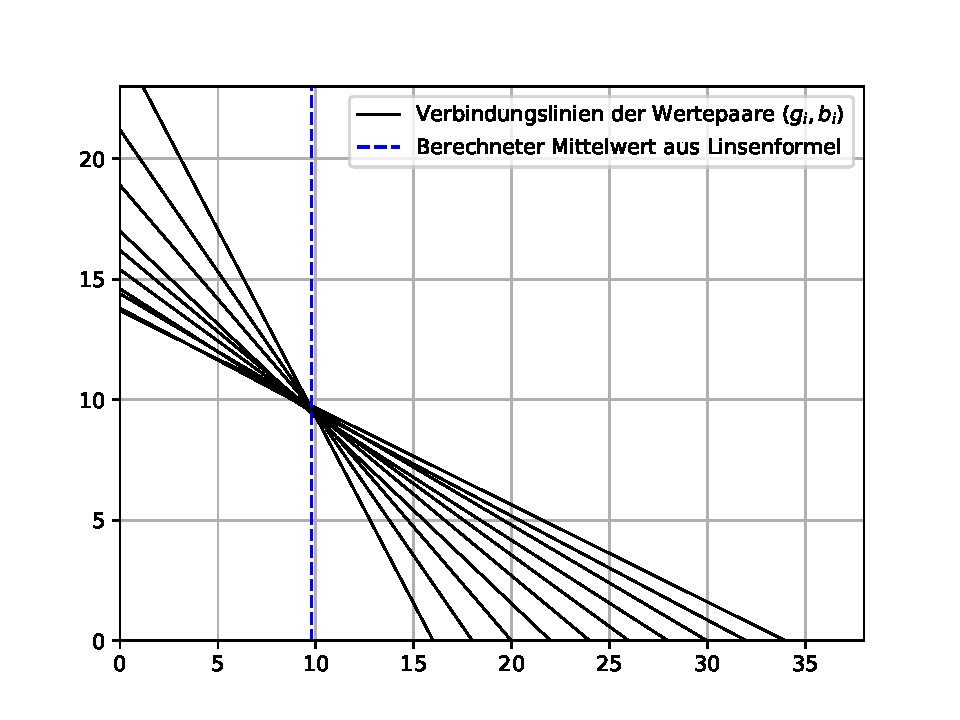
\includegraphics[width=0.7\textwidth]{../Messdaten/plots/methode_1.pdf}
  \caption{Darstellung der Verbindungsgeraden $(g\ua{i}, 0) - (0, b\ua{i})$ zur Bestimmung der Brennweite einer
  Linse bekannter Brennweite $f = \SI{100}{\centi\meter}$.}
  \label{fig: methode_1}
\end{figure}
\begin{table}
\centering
\caption{Messdaten zur Überprüfung der Abbildungs- \eqref{eq: abbildungsgesetz_gross} und Linsengleichung \eqref{eq: linsengleichung}.}
\label{tab: methode_1}
\begin{tabular}{S[table-format=2.1]@{${}\pm{}$} S[table-format=1.1]
S[table-format=2.1]@{${}\pm{}$} S[table-format=1.1]
S[table-format=1.1]@{${}\pm{}$} S[table-format=1.1]
S[table-format=1.2]@{${}\pm{}$} S[table-format=1.2]
S[table-format=1.2]@{${}\pm{}$} S[table-format=1.2]
S
 }
\toprule
\multicolumn{2}{c}{$g \:/\: \si{\centi\meter}$} &
\multicolumn{2}{c}{$b \:/\: \si{\centi\meter}$} &
\multicolumn{2}{c}{$B \:/\: \si{\centi\meter}$} &
\multicolumn{2}{c}{$V_1$} &
\multicolumn{2}{c}{$V_2$} &
{$\left(\frac{V_2}{V_1} - 1\right) \:/\: \si{\percent}$} \\
\midrule
 16.0  & 0.1  & 24.8  & 0.1  & 4.6  & 0.1  & 1.53  & 0.06  & 1.55  & 0.01  & -0.01\\
18.0  & 0.1  & 21.2  & 0.1  & 3.6  & 0.1  & 1.20  & 0.05  & 1.18  & 0.01  & 0.02\\
20.0  & 0.1  & 18.9  & 0.1  & 2.9  & 0.1  & 0.97  & 0.05  & 0.94  & 0.01  & 0.02\\
22.0  & 0.1  & 17.0  & 0.1  & 2.4  & 0.1  & 0.80  & 0.04  & 0.77  & 0.01  & 0.04\\
24.0  & 0.1  & 16.2  & 0.1  & 2.2  & 0.1  & 0.73  & 0.04  & 0.67  & 0.01  & 0.09\\
26.0  & 0.1  & 15.4  & 0.1  & 1.9  & 0.1  & 0.63  & 0.04  & 0.59  & 0.00  & 0.07\\
28.0  & 0.1  & 14.6  & 0.1  & 1.8  & 0.1  & 0.60  & 0.04  & 0.52  & 0.00  & 0.15\\
30.0  & 0.1  & 14.4  & 0.1  & 1.6  & 0.1  & 0.53  & 0.04  & 0.48  & 0.00  & 0.11\\
32.0  & 0.1  & 13.8  & 0.1  & 1.5  & 0.1  & 0.50  & 0.04  & 0.43  & 0.00  & 0.16\\
34.0  & 0.1  & 13.7  & 0.1  & 1.4  & 0.1  & 0.47  & 0.04  & 0.40  & 0.00  & 0.16\\
\bottomrule
\end{tabular}
\end{table}


\subsection{Bestimmung der Brennweite einer unbekannten Linse}
Nach der selben Methode wie im vorangegangen Abschnitt wird die Brennweite einer unbekannten Linse bestimmt.
Die aufgenommen Daten sind in Tabelle \ref{} eingefügt. Die Graphische Darstellung der Verbindungslinien ist
in Abbildung \ref{fig: wasserlinse} einzusehen. Mit der Linsenformel ergibt sich durch Mittelung der Wert
\begin{equation}
  f\ua{u, mid} = \SI{+13.83(1)}{\centi\meter}
\end{equation}
Aus dem Graphen \ref{fig: wasserlinse} wird folgender Schnittpunkt abgelesen
\begin{equation}
  f\ua{u, exp} = \SI{14.1(1)}{\centi\meter}.
\end{equation}
\begin{table} 
\centering 
\caption{Messdaten zur Bestimmung der Brennweite einer unbekannten Linse, Gegenstandsweite $g$ und Bildweite $b$.} 
\label{tab: wasserlinse} 
\begin{tabular}{S[table-format=2.1]@{${}\pm{}$} S[table-format=1.1]
S[table-format=2.1]@{${}\pm{}$} S[table-format=1.1]
 } 
\toprule  
\multicolumn{2}{c}{$g \:/\: \si{\centi\meter}$} & \multicolumn{2}{c}{$b \:/\: \si{\centi\meter}$}  \\ 
\midrule  
 20.0  & 0.1  & 47.3  & 0.1\\ 
21.0  & 0.1  & 41.3  & 0.1\\ 
22.0  & 0.1  & 36.8  & 0.1\\ 
23.0  & 0.1  & 34.5  & 0.1\\ 
24.0  & 0.1  & 31.4  & 0.1\\ 
25.0  & 0.1  & 32.3  & 0.1\\ 
30.0  & 0.1  & 25.5  & 0.1\\ 
35.0  & 0.1  & 22.3  & 0.1\\ 
\bottomrule 
\end{tabular} 
\end{table}

\begin{figure}
  \centering
  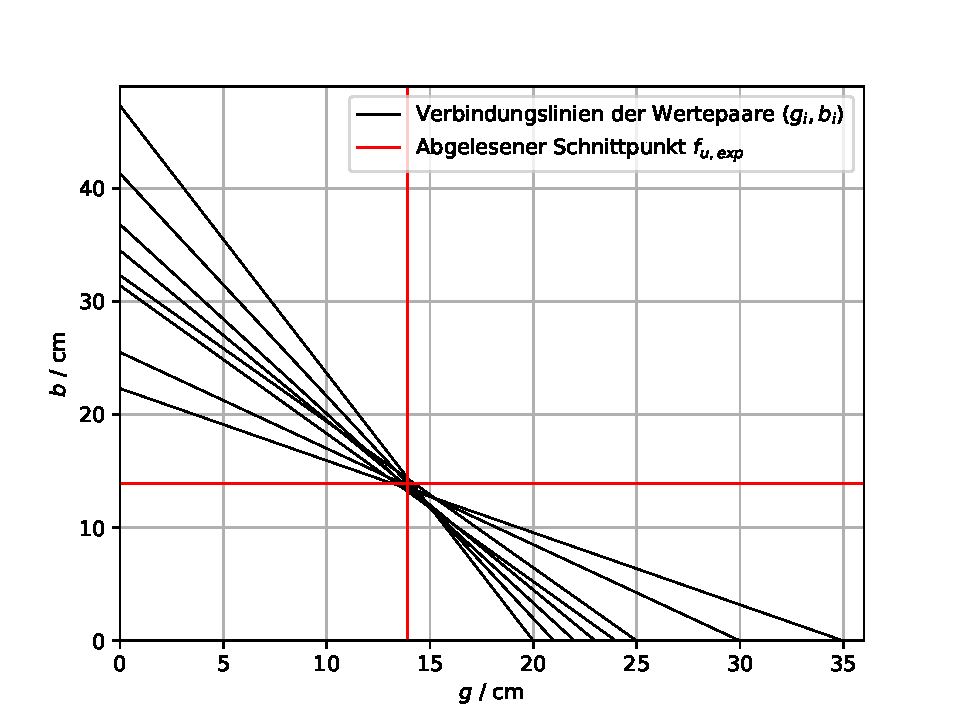
\includegraphics[width = 0.7\textwidth]{../Messdaten/plots/wasserlinse.pdf}
  \caption{Darstellung der Verbindungsgeraden $(g\ua{i}, 0) - (0, b\ua{i})$ zur Bestimmung der Brennweite einer
  Linse unbekannter Brennweite.}
  \label{fig: wasserlinse}
\end{figure}

\subsection{Bestimmung der Brennweite nach der Methode von Bessel}
Die gemessenen Werte für die beiden Punkte $(g_1, b_1)$ und $(g_2, b_2)$, bei denen unter konstantem Abstand
zwischen Schirm und Gegenstand jeweils Bild und Gegenstandsweite
vertauschen, sind in Tabelle \ref{tab: bessel} einzusehen. Mit Gleichung \eqref{} ergibt sich der Mittelwert für
die Brennweite $f\ua{2, mid}$ zu
\begin{equation}
  f\ua{2, mid} = \SI{+9.90(1)}{\centi\meter}.
\end{equation}
\begin{table}[H] 
\centering 
\caption{Messdaten zur Bestimmung der Brennweite mit der Methode nach Bessel.} 
\label{tab: bessel} 
\begin{tabular}{S S S S S S } 
\toprule  
{$g_1 / \si{\centi\meter}$} & {$b_1 / \si{\centi\meter}$} &{$g_2 / \si{\centi\meter}$} &  {$b_2 / \si{\centi\meter}$} & {$f_1 / \si{\centi\meter}$} & {$f_2 / \si{\centi\meter}$}  \\ 
\midrule  
 22.8  & 17.2  & 16.7  & 23.3  & 9.8  & 9.7\\ 
27.8  & 15.2  & 14.9  & 28.1  & 9.8  & 9.7\\ 
34.3  & 13.7  & 13.6  & 34.4  & 9.8  & 9.7\\ 
39.7  & 13.3  & 13.1  & 39.9  & 10.0  & 9.9\\ 
45.2  & 12.8  & 12.2  & 45.8  & 10.0  & 9.6\\ 
50.5  & 12.5  & 12.4  & 50.6  & 10.0  & 10.0\\ 
55.7  & 12.3  & 12.0  & 56.0  & 10.1  & 9.9\\ 
60.8  & 12.2  & 11.8  & 61.2  & 10.2  & 9.9\\ 
66.2  & 11.8  & 11.7  & 66.3  & 10.0  & 9.9\\ 
71.2  & 11.8  & 11.5  & 71.5  & 10.1  & 9.9\\ 
\bottomrule 
\end{tabular} 
\end{table}
